%
% randwerte.tex -- 
%
% (c) 2015 Prof Dr Andreas Mueller, Hochschule Rapperswil
%
\section{Randwertprobleme\label{section:numerik:randwertprobleme}}
\rhead{Randwertprobleme}
Die bisher beschriebenen Verfahren gehen von einer Anfangsbedingung
aus, und berechnen die dadurch eindeutig festgelegte Lösungskurve.
Randwertproblem, beschrieben in Abschnitt~\ref{section:randwertprobleme},
verknüpfen dagegen Werte von einzelnen Komponenten von $Y$ an den
Rändern eines Intervalls.
\index{Randwertproblem}%

\subsection{Einführende Beispiele}
Wir betrachten zwei prototypische Randwertprobleme, die das allgemeine
Lösungsverfahren motivieren sollen.
In der ersten Aufgabe sind wir dank einer expliziten Form der Lösung
nach Einsetzen der Randwertbedingung die Parameter durch Lösen
von Gleichungen zu bestimmen.

%\newtheorem{aufgabe}{Aufgabe}[chapter]
\begin{aufgabe}
\label{numerik:aufgabe-ball}
Mit einem nur der Schwerkraft unterworfenen Ball, der im Ursprung des
Koordinatensystems geworfen wird, soll ein Ziel im Punkt $P$ getroffen
werden.
In welcher Richtung und mit welcher Anfangsgeschwindigkeit muss er geworfen
werden?
\end{aufgabe}

Um das Problem einfach zu halten, modellieren wir diese Aufgabe wie
folgt.
Der Ball der Masse $m$ bewegt sich in der $x$-$y$-Ebene, wobei die
Schwerkraft in negativer $y$-Richtung zeigt.
Das Newtonsche Gesetz liefert die Differentialgleichung zweiter Ordnung
\begin{equation}
m\frac{d^2}{dt^2}\begin{pmatrix}x\\y\end{pmatrix}
=
\begin{pmatrix}
0\\-mg
\end{pmatrix}.
\label{numerik:ball-dgl}
\end{equation}
Die Masse $m$ kann herausgekürzt werden.
Gesucht ist eine Lösung so, dass die Bahn durch die Punkte $(0,0)$
und $P=(p,0)$ geht.

Genau genommen ist dies nicht ein Randwertproblem wie in 
Abschnitt~\ref{section:randwertprobleme}, denn es wird nicht verlangt,
dass der Ball zu einer bestimmten Zeit $t$ beim Punkt $P$ eintrifft.
Die Differentialgleichung bedeutet aber, dass die Horizontalgeschwindigkeit
des Balls konstant ist (die horizontale Beschleunigung ist immer $0$).
Ist $v_x$ die Horizontalgeschwindigkeit, dann erreicht der Ball zur
Zeit $t_1=p/v_x$ die $x$-Koordinate des Ziels.
Gesucht ist also die anfängliche Vertikalgeschwindigkeit, die man
dem Ball geben muss, dass zur Zeit $p/v_x$ die $y$-Komponente
der Lösung den Wert $0$ hat.
In dieser Form liegt ein Randwertproblem wie in
Abschnitt~\ref{section:randwertprobleme} vor.

Die Lösungen der Differentialgleichung~\ref{numerik:ball-dgl} sind aus
dem Physik-Unterricht bekannt:
es gilt
\begin{equation}
\begin{pmatrix}x(t)\\y(t)\end{pmatrix}
=
\begin{pmatrix}v_xt\\ v_yt-\frac12gt^2\end{pmatrix}
\end{equation}
Damit lässt sich auch das Randwertproblem lösen.
Für $t=v_x/p$ muss $y(t)=0$ sein, also
\begin{align}
y(t)=y\biggl(\frac{p}{v_x}\biggr)
=v_y\frac{p}{v_x}-\frac12g\biggl(\frac{p}{v_x}\biggr)^2&=0
\notag
\\
\Rightarrow\qquad
v_y
&=
\frac{v_x}p\frac12g\frac{p^2}{v_x^2}=\frac{gp}{2v_x}.
\label{numerik:ball-bedingung}
\end{align}
Offenbar gibt es zu jedem $v_x$ einen passenden Wert von $v_y$,
mit dem das Ziel getroffen wird.

Die Differentialgleichung \eqref{numerik:ball-dgl} ist nicht in einer
Form, die der numerischen Lösung zugänglich ist.
Wir schreiben Sie daher als Differentialgleichung erster Ordnung 
für vierdimensionale Vektoren:
\begin{align}
\frac{d}{dt}Y
=
\frac{d}{dt}\begin{pmatrix}x\\y\\\dot x\\\dot y\end{pmatrix}
&=
\begin{pmatrix}\dot x\\\dot y\\ 0\\ -g\end{pmatrix}.
\label{numerik:ball-dgl-1}
\end{align}
Gesucht ist eine Lösung, die die Randbedingungen
\begin{equation}
Y(0)
=
\begin{pmatrix}0\\0\\v_x\\\color{red}v_y\end{pmatrix},
\qquad
Y\biggl(\frac{p}{v_x}\biggr)
=
\begin{pmatrix}p\\0\\\color{red}?\\\color{red}?\end{pmatrix}
\label{numerik:ball-dgl-2}
\end{equation}
erfüllt.
Darin stehen die roten Einträge für Werte, die nicht vorgegeben sind.
Aus der Symmetrie des Problems kann man natürlich auch die Endgeschwindigkeit
ablesen.
Zu bestimmen ist also $v_y$ so, dass die Lösungskurve durch den Punkt
$(p,0)$ geht.

Wird statt der Horizontalkomponenten der Anfangsgeschwindigkeit die
gesamte Anfangsgeschwindigkeit $v_0$ vorgegeben, dann muss der
Winkel gefunden werden, unter dem der Ball geworfen werden muss,
um das Ziel zu trefen.
Bei der Elevation $\alpha$ sind die Komponenten der Anfangsgeschwindigkeit
$v_x=v_0\cos\alpha$ und $v_y=v_0\sin\alpha$. 
Setzt man dies in die Bedingung~\eqref{numerik:ball-bedingung} ein,
findet man
\begin{align*}
v_0 \sin \alpha &=\frac{gp}{2v_0\cos\alpha}
\\
2\sin\alpha\cos\alpha&=\frac{gp}{v_0^2}
\\
\sin2\alpha&=\frac{gp}{v_0^2}
\\
\alpha&= \frac12 \arcsin\frac{gp}{v_0^2}.
\end{align*}
Im Nenner rechts steht im wesentlichen die kinetische Energie,
je mehr kinetische Energie der Ball zu Beginn hat, desto kleiner
ist der Winkel, man trifft das Ziel mit einer sehr flachen Bahn.
Kleine Winkel reichen auch für geringe Schwerkraft ($g$ klein)
und kurze Distanzen ($p$ klein).
Die maximale Distanz wird erreicht, wenn das Argument des Arcussinus
den Wert $1$ erreicht, grösser darf $p$ nicht werden, weil es sonst
keine Lösung mehr für $\alpha$ gibt.
Die Maximaldistanz ist daher
\[
p_{\text{max}} = \frac{v_0^2}{g}.
\]

\begin{aufgabe}
\label{numerik:aufgabe-seil}
Ein Seil ist zwischen zwei Punkten aufgehängt, welche Form nimmt es
allein unter der Wirkung seines Eigengewichtes an?
\end{aufgabe}
Die Lösungskurve dieses Problems heisst die {\em Kettenlinie}.
\index{Kettenlinie}
Auch in diesem Fall können wir wieder eine Lösungsfunktion $y(x)$ finden,
aber die Bestimmung der Parameter ist jetzt nicht mehr in geschlossener
Form möglich.
Wir behelfen uns mit einer numerischen Lösung.

\begin{loesung}
\def\asinh{\operatorname{asinh}}
\begin{figure}
\centering
%\includegraphics{chapters/images/numerik-5.pdf}
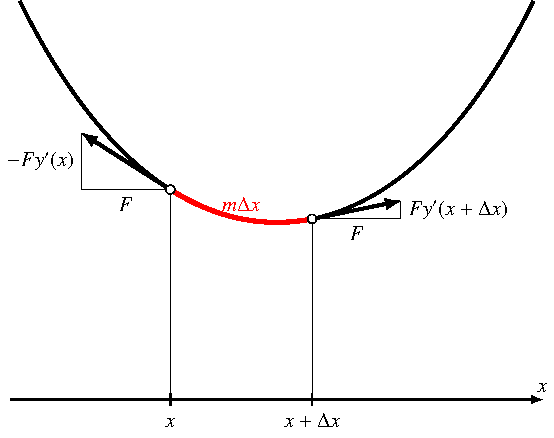
\includegraphics{chapters/50-ode/figures/kettenlinie.pdf}
\caption{Herleitung der Differentialgleichung der Kettenlinie
\label{numerik:kettenlinie}}
\end{figure}
Zunächst brauchen wir für eine Differentialgleichung, deren Lösung die
gesuchte Kurve beschreibt.
Zur Herleitung dient die Abbildung~\ref{numerik:kettenlinie}.
Die Masse des Seils zwischen den beiden Punkten $x$ und $x+\Delta x$
wird von den beiden eingezeichneten Kräften getragen.
Die horizontalen Komponenten tragen nicht dazu bei, das Seil zu
tragen, sie haben daher entlang des ganzen Seils immer die gleiche
Grösse $F$.
Die Masse des Seilstücks ist proportional zu seiner Länge,
der Proportionalitätsfaktor ist die lineare Massendichte $\mu$.
Nach dem dritten Newtonschen Gesetz
\index{Newton!drittes Gesetz von}
sind die vertikalen Kraftkomponenten gleich gross wie die Gewichtskraft
des Seilstücks:
\begin{align*}
F(y'(x+\Delta x)-y'(x))
&= \mu g\sqrt{(y(x+\Delta x)-y(x))^2+\Delta x^2}
\\
\intertext{oder nach Divison durch $F\Delta x$:}
\frac{y'(x+\Delta x)-y'(x)}{\Delta x}
&=\frac{\mu g}{F}\sqrt{1+\biggl(\frac{y(x+\Delta x)-y(x)}{\Delta x}\biggr)^2}.
\end{align*}
Schreibt man $a=\mu g/F$ und geht zur Grenze $\Delta x\to 0$ über,
erhält man die Differentialgleichung
\begin{equation}
y''(x)=a\sqrt{1+y'(x)^2}.
\label{numerik:kettenloesung}
\end{equation}
Diese Differentialgleichung hat die Funktion
\[
y(x) = \frac1a \cosh ax + C
\]
als Lösung, wie man durch Nachrechnen einsehen kann\footnote{
Man kann die Gleichung~\eqref{numerik:kettenloesung} natürlich auch direkt
lösen. Dazu bestimmt man zuerst die Funktion $z(x)=y'(x)$, welche die
Differentialgleichung
\[
z'(x)=a\sqrt{1+z(x)^2}
\]
erfüllt.
Diese Gleichung lässt sich durch Separation lösen:
\[
\begin{aligned}
\frac{dz}{dx}&=a\sqrt{1+z^2}
&&\Rightarrow&
\frac1a \int\frac{dz}{\sqrt{1+z^2}}&=\int \,dx
&&\Rightarrow&
\frac1a \asinh z &=x+C_1
&&\Rightarrow&
z(x)=\sinh a(x+C_1).
\end{aligned}
\]
Die Funktion $y(x)$ bekommt man jetzt durch Integration
\[
y(x)=\int z(x)\,dx = \frac1a \cosh a(x+C_1) + C_2,
\]
mit $C_1 = -x_0$ und $C_2=C$ genau die vorgeschlagene Lösung.
}.
Die Ableitungen von $y(x)$ sind
\begin{align*}
y' (x) &=  \sinh ax\\
y''(x) &= a\cosh ax.
\end{align*}
Eingesetzt in die Differentialgleichung erhält man
\begin{align*}
a\cosh ax&=a\sqrt{1+\sinh^2 ax},
\\
\intertext{was sich zu}
\cosh^2ax-\sinh^2ax&=1
\end{align*}
umformen lässt, diese Gleichung ist für hyperbolische Funktionen
immer erfüllt.

Die Differntialgleichung~\eqref{numerik:kettenloesung}
ist autonom, also sind auch verschobene Funktionen Lösungen.
Die allgemeine Lösung des Problems ist daher die Funktion
\begin{equation}
y(x)=\frac1a\cosh a(x-x_0) + C.
\label{numerik:ketteaC}
\end{equation}
Die Bedeutung der Konstante $C$ ist leichter verständlich, wenn man sie
als $C=y_0-1/a$ schreibt, also
\[
y(x)=\frac1a\cosh a(x-x_0) -\frac1a+y_0.
\]
Setzt man $x=x_0$ ein, findet man $y(x_0)=y_0$, d.~h.~der Punkt $(x_0,y_0)$
ist der Scheitelpunkt des Graphen von $y(x)$.

Damit kann jetzt das Anfangswertproblem gelöst werden.
Wir verlangen, dass die im Punkt $x=x_1$ der Funktionswert 
$y(x_1)=y_1$ sein soll, und die Steigung $y'(x_1)=m$.
Setzt man die Lösung~\eqref{numerik:ketteaC} in die Bedingung
für die Steigung ein, erhält man
\[
m=\sinh a(x_1-x_0)
\qquad\Rightarrow\qquad
\asinh m =a(x_1-x_0)
\qquad\Rightarrow\qquad
x_0=x_1-\frac1a\asinh m.
\]
Die Anfangsbedingung für $y(x_1)$ liefert
\begin{align*}
y_1
&=
y(x_1)
=
\frac1a\cosh a(x_1-x_0) + y_0 - \frac1a
=
\frac1a\cosh \asinh(m)+y_0-\frac1a
=
\frac1a\sqrt{1+m^2}+y_0-\frac1a
\\
\Rightarrow\quad
y_0
&= 
y_1+\frac1a-\frac1a\sqrt{1+m^2}.
\end{align*}
Damit ist das Anfangswertproblem vollständig gelöst, 
\begin{equation}
y(x)
=
\frac1a\cosh \bigl(a(x-x_1) + \asinh m\bigr)
+ y_1 - \frac1a\sqrt{1+m^2}
\end{equation}
ist die allgemeine Lösung zur Anfangsbedingung $y(x_1)=y_1$, $y'(x_1)=m$.

Mit dieser Lösung kann jetzt auch das Randwertproblem gelöst werden.
Es muss ein Wert $m$ gefunden werden, so dass $y(x_2)=y_2$,
man muss also die Gleichung
\[
y_2
=
\frac1a\cosh \bigl(a(x_2-x_1)+\asinh m\bigr) + y_1 - \frac1a\sqrt{1+m^2}
=:
f(m)
\]
nach $m$ auflösen.
Das ist leider nicht so einfach, weil $m$ in der transzendenten Funktion
$\asinh$ auftritt.

Wir können die Gleichung jedoch iterativ mit dem Newton-Verfahren
nach Satz~\ref{newton:satz} lösen.
Dazu brauchen wir die Ableitung von $f$, sie ist
\[
f'(m)
=
\frac{ \sinh (x_2-x_1+\asinh m) -m}{\sqrt{m^2+1}}.
\]
Damit können wir die Iterationsformel
\[
m_{\text{neu}} = m - \frac{f(m) - y_2}{f'(m)}
\]
für den korrekten Wert $m$ finden.
Sie kann leicht in Octave implementiert werden, wie Listing~\ref{numerik:ketteprog} zeigt.
%\lstinputlisting[style=Octave]{chapters/examples/kette.m}
%\begin{lstlisting}[style=Octave,caption={Octave-Programm zur Bestimmung der Anfangssteigung $m$ im Kettenlinien-Problem}]
%\begin{lstlisting}[style=Octave, caption={Octave-Programm}, captionpos={b}, label={numerik:ketteprog}]
%\verbatiminput{chapters/examples/kette.m}

In Tabelle~\ref{numerik:kette-newton} ist der Gang der Berechnung
für den Fall $x_1=-1$, $x_2=2$, $y_1=1$ und $y_2=2$  mit dem
Startwert $m=0$ dargestellt.
Wie erwartet ist die Konvergenz quadratisch, in jedem Schritt verdoppelt
sich die Anzahl korrekter Stellen.
In Abbildung~\ref{numerik:kette-newton-graph} sind die Graphen von $y(x)$
zu den im Newton-Algorithmus ermittelten Werten von $m=y'(x_1)$ blau
dargestellt, die Lösungskurve ist rot.
\begin{table}
\centering
\begin{tabular}{|r|>{$}c<{$}|>{$}c<{$}|}
\hline
  &                      m                 &           f(m)               \\
\hline
 1&\phantom{-}           0.0000000000000000& \phantom{-}8.0676619957777653\\
 2&         -            0.8053266839760436& \phantom{-}2.5748454835378896\\
 3&         -\underline{1}.3999183852140562& \phantom{-}0.5757860863682827\\
 4&         -\underline{1.6}180720459804230& \phantom{-}0.0383682292517731\\
 5&         -\underline{1.634}7219547661627& \phantom{-}0.0001812733120350\\
 6&         -\underline{1.63480136}59846743& \phantom{-}0.0000000040625958\\
 7&         -\underline{1.634801367764473}7& \phantom{-}0.0000000000000004\\
 8&         -\underline{1.6348013677644739}&           -0.0000000000000002\\
\hline
\end{tabular}
\caption{Numerische Lösung des Randwertproblems für die Kettenlinie
mit Randbedingungen $x_1=-1$, $x_2=2$, $y(x_1)=y_1$ und $y(x_2)=y_2$.
\label{numerik:kette-newton}}
\end{table}
\begin{figure}
\centering
%\includegraphics[width=\hsize]{chapters/images/numerik-6.pdf}
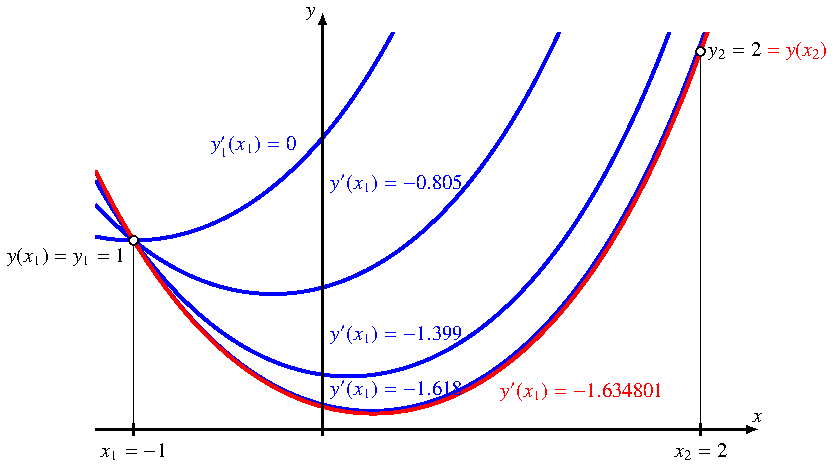
\includegraphics{chapters/50-ode/figures/kettenloesung.pdf}
\caption{Iterative Bestimmung der Kettenlinie zwischen
den Punkten $(-1,2)$ und $(2,2)$ mit Hilfe des Newton-Algorithmus.
\label{numerik:kette-newton-graph}}
\end{figure}
\end{loesung}
\begin{lstlisting}[style=Octave,caption={Octave-Programm zur Bestimmung der Anfangssteigung $m$ im Kettenlinien-Problem}, captionpos={t}, label={numerik:ketteprog}]
global x1 = -1
global x2 =  2
global y1 =  1
global y2 =  2

function v = f(m)
        global x1 x2 y1 y2
        v = cosh(x2 - x1 + asinh(m)) + y1 - y2 - sqrt(1 + m^2);
endfunction

function v = fprime(m)
        global x1 x2 y1 y2
        v = (sinh(x2 - x1 + asinh(m)) - m)/sqrt(1 + m^2);
endfunction

m = 0;

for i = (1:10)
        printf("%2d   %20.16f %20.16f\n", i, m, f(m));
        m = m - f(m)/fprime(m);
endfor
\end{lstlisting}

\subsection{Schiess-Verfahren\label{numerik:schiess-verfahren}}
\index{Schiess-Verfahren}%
Wenn man experimentell versucht, ein Ziel zu treffen, dann wird man
in wiederholten Versuchen die Richtung anpassen, so dass man dem Ziel
immer näher kommt.
Genau dies haben wir in der Aufgabe~\ref{numerik:aufgabe-seil} gemacht,
wo wir iterativ die noch unbekannen Anfangsbedingung $y(x_1)=m$ bestimmt
haben, mit der die Lösung durch den rechten Randpunkt $y(x_2)=y_2$ geht.

Auch in der Aufgaben~\ref{numerik:aufgabe-ball} konnten wir die
Parameter direkt bestimmen.
Doch auch dort läuft die Lösung auf die Bestimmung einer 
geeigneten Anfangsbedingung hinaus.
Der $y$-Wert zur Zeit $p/v_x$ hängt von der Vertikalgeschwindigkeit ab,
wir bezeichnen ihn mit $h(v_y)$.
Man verändert also $v_y$, bis die Gleichung $h(v_y)=0$ erfüllt ist.
Um das Randwertproblem zu lösen, muss man also die Gleichung $h(v_y)=0$
numerisch lösen.

Man kann dies z.~B.~dadurch machen, dass man nach zwei Werten von $v_y$
sucht, so dass die zum einen gehörige Bahn unter dem Punkt $P$ durchgeht,
während der Ball im anderen Fall darüber hinwegfliegt.
Durch wiederholte Halbierung des Intervalls kann man dann den korrekten
Wert für $v_y$ immer genauer eingrenzen%
\footnote{%
Tatsächlich wird dieses Verfahren in der Artillerie verwendet.
\index{Artillerie}%
Der Schiesskommandant beobachtet die einschlagenden Granaten und kommandiert
Änderungen der Anfangs-Elevation an die Geschützbatterien.
Dabei sucht er Einschläge, die aus seiner Perspektive vor bzw.~hinter
dem Ziel liegen, und halbiert dann das Intervall, bis die Einschläge dem
Ziel genügend nahe kommen.}.
Der Nachteil dieses Verfahrens ist, dass mit jedem Schritt die Genauigkeit
nur um in Bit ansteigt, es sind also sehr viele Iterationen notwendig.

Schnellere Konvergenz kann mit dem Newton-Verfahren erreicht werden,
welches in Anhang~\ref{chapter:newton} beschrieben wird.
\index{Newton-Verfahren}%
Für die Anwendung des Newton-Verfahrens auf das Randwert-Problem
ist die Bestimmung der Steigung der Funktion nötig, die die Abweichung
der Kurve von der Randbedingung am rechten Rand angibt.
Wir müssen also berechnen, wie schnell sich $y(p/v_x)$ ändert,
wenn $v_y$ verändert wird.
Dies ist die Ableitung
\[
h'(v_y)= \frac{\partial y}{\partial v_y},
\]
ein Eintrag der Jacobi-Matrix.
In Abschnitt~\ref{grundlagen:jacobi} wurde gezeigt, wie man auch für
die Jacobi-Matrix eine Differentialgleichung aufstellen kann, die
man natürlich ebenfalls mit den früher beschriebenen numerischen
Bibliotheken lösen kann.

Das Randwertproblem kann daher mit folgendem Algorithmus numerisch gelöst
werden.
\begin{enumerate}
\item Beginne mit einer Schätzung für $v_y$
\item Finde numerisch die Lösung des Anfangswertproblems mit $v_y$
als anfängliche Vertikalgeschwindigkeit.
Berechnet dabei auch die Jacobi-Matrix
\item Lese die $h(v_y)$ aus der Lösung zur Zeit $p/v_x$ ab, und $h'(v_y)$
aus der Jacobi-Matrix und verwendet den Newton-Algorithmus
(Satz~\ref{newton:satz}), um eine verbesserte Schätzung von $v_y$ 
zu bekommen.
\item Wiederhole Schritte 2 und 3 bis die Randbedingung für $t=p/v_x$
genügend genau erfüllt ist.
\item Die Lösung des Anfangswertproblems mit diesem $v_y$ ist die
Lösung des gestellten Randwertproblems.
\end{enumerate}

\begin{beispiel}
\begin{figure}
\centering
%\includegraphics{chapters/images/randwert-1.pdf}
\caption{Lösungen des Anfangswertproblems~\eqref{numerik:ball-dgl-1} und
\eqref{numerik:ball-dgl-2}.
Das Newton-Verfahren korrigiert $v_y$ derart, dass $h(v_y)=0$ wird.
So wird die Lösung des Randwertproblems (rot) gefunden.
\label{numerik:randwert-bild}}
\end{figure}
Wir führen den eben skizzierten Algorithmus für das Ball-Problem durch.
Um die Jacobi-Matrix zu berechnen, müssen wir die Ableitung von $f$ berechnen:
\begin{equation}
\frac{\partial f(x,y)}{\partial y}
=
\begin{pmatrix}
0& 0& 1& 0\\
0& 0& 0& 1\\
0& 0& 0& 0\\
0& 0& 0& 0
\end{pmatrix}.
\end{equation}
Da die rechte Seite nicht von $y$ abhängt, können wir die Gleichung für
die Jacobi-Matrix ganz unabhängig von $y$ lösen.
Da $F$ so einfach ist, kann man das Matrizenprodukt direkt ausrechnen, 
so wird die Differentialgleichung für $J$
\begin{equation}
\begin{pmatrix}
J'_{11}&J'_{12}&J'_{13}&J'_{14}\\
J'_{21}&J'_{22}&J'_{23}&J'_{24}\\
J'_{31}&J'_{32}&J'_{33}&J'_{34}\\
J'_{41}&J'_{42}&J'_{43}&J'_{44}
\end{pmatrix}
=
\begin{pmatrix}
0& 0& 1& 0\\
0& 0& 0& 1\\
0& 0& 0& 0\\
0& 0& 0& 0
\end{pmatrix}
\begin{pmatrix}
J_{11}&J_{12}&J_{13}&J_{14}\\
J_{21}&J_{22}&J_{23}&J_{24}\\
J_{31}&J_{32}&J_{33}&J_{34}\\
J_{41}&J_{42}&J_{43}&J_{44}
\end{pmatrix}
=
\begin{pmatrix}
J_{31}&J_{32}&J_{33}&J_{34}\\
J_{41}&J_{42}&J_{43}&J_{44}\\
     0&     0&     0&     0\\
     0&     0&     0&     0
\end{pmatrix}.
\end{equation}
\begin{table}
\centering
\begin{tabular}{|>{$}r<{$}|>{$}r<{$}|>{$}r<{$}|>{$}r<{$}|>{$}r<{$}|>{$}r<{$}|>{$}r<{$}|>{$}r<{$}|}
\hline
n&    v_y&    t& x(t)&      y(x)&\displaystyle\frac{\partial^{\mathstrut}y}{\partial v_y}&v_{y,\text{new}}&\Delta\\
\hline
0& 7.0000&  2.5& 20.0&-13.156250&  2.5& 12.26250000& -5.2625000000\\
1&12.2625&  2.5& 20.0& -0.000004&  2.5& 12.26250145& -0.0000014458\\
2&12.2625&  2.5& 20.0&  0.000000&  2.5& 12.26250143&  0.0000000204\\
\hline
\end{tabular}
\caption{Newton-Algorithmus für das Ball-Problem, Resultate der numerischen
Rechnung.
$v_y$ wird in drei Schritten mit einer Genauigkeit von mehr als 10 Stellen
gefunden.
\label{numerik:newton-resultate}}
\end{table}%
Daraus kann man ablesen, dass die Elemente $J_{3j}$ und $J_{4j}$ sich
nicht ändern, sie bleiben also konstant.
Aber auch in den ersten zwei Zeilen können sich nur die Elemente $J_{13}$
und $J_{24}$ ändern, die Differentialgleichungen für diese Elemente
sind
\begin{align*}
J'_{13}&=1\\
J'_{24}&=1
\end{align*}
oder in Matrixform:
\begin{equation}
J(x) = \begin{pmatrix}
1&0&x&0\\
0&1&0&x\\
0&0&1&0\\
0&0&0&1
\end{pmatrix}.
\end{equation}
Die Lösung $J_{13}(x)=x$ und $J_{24}=x$.
Damit haben wir die nötige Information, um den Newton-Algorithmus
durchzuführen.
In Tabelle~\ref{numerik:newton-resultate}
sind die Resultate der numerischen Rechnung zusammengestellt.
Es zeigt sich, dass der korrekte Wert für $v_y$ in drei Iterationen
mit 10 Stellen Genauigkeit gefunden werden kann.
Damit ist das Randwertproblem numerisch gelöst.
\end{beispiel}
